\chapter{Background}\label{ch:background}
% Include only work that is addressing the same or a very similar goal as
% yours.  First, explain what the other authors did in their work in your
% own words. Then discuss why you solved the same problem differently.
%
% There is plenty of work on network switching and buffer architecture

The objective of a flow-aware packet buffer is to temporarily store incoming packets and organize them by flows so that different consumers 
can ingest them. Let us consider the case of a network switch as an example where there are many output interfaces operating at the same time and 
each of them has provides access to a different subset of the network. If packet from flow A and B have to be routed through a different physical 
interface each to reach their destinations, then an agent needs to separate the flows so that they can be routed accordingly. This is in 
essence the job of a flow-aware packet buffer. \\

Before presenting the proposed design, this section reviews existing approaches described in the literature. 
Particularly, it covers the shared-memory architecture, which is a widely used approach to buffering 
and rerouting packets in a network processor. That being said, there are specific challenges that are unique 
to the problem described in the introduction chapter \ref{ch:introduction} which will 
be discussed here as well.

\section{The shared-memory architecture}
%Here we explain the behavior of a shared-memory architecture for a router/packet buffer.
As stated previously, there is research on packet buffer architecture \cite{inproceedings} and their application 
in a specific context, \cite{lau2003gigabit} \cite{naous2008netfpga}. For the purposes of this work, the paper published 
by Queens University Belfast \cite{inproceedings} is particularly relevant as it defines and implements a generic shared 
packet buffer design. \\

The proposed design follows a shared-memory architecture, which uses a common pool of memory where all packets are stored, instead of 
buffering the packets in a per-flow basis where every flow has its own dedicated memory. Then, logical queues store pointers to the packets 
stored in the memory, which keeps track of which packets belong to which flow; and a different queue stores pointers to unallocated memory 
locations. This way, when a packet arrives an unallocated memory location is popped, the data from said packet is written in that region, 
and the pointer to the region is pushed to the respective flow queue. When a packet needs to be consumed, the inverse process takes place, 
where a packet address is popped from the respective flow queue, the packet is read, and the memory space (now free) is returned to the 
unallocated location queue. Figure \ref{fig:shared-buffer} shows 
an overview of this architectural approach. \\

\begin{figure}
  \begin{center}
    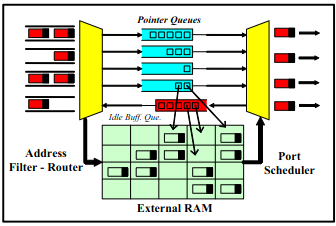
\includegraphics[width=0.95\textwidth]{../img/shared-buffer.png}
  \end{center}
  \caption{Shared-memory architecture (source \cite{inproceedings})}\label{fig:shared-buffer}
\end{figure}

All in all, the architecture is essentially a dynamically allocated pool of fixed-size memory blocks combined with logical packet 
queues and buffer-management pointers, allowing variable-length packets from multiple queues to share the same physical memory. \\

Using descriptor queues instead of buffering packet data directly on a per-flow basis provides better memory utilization and greater flexibility since each flow 
only maintains a small queue of descriptors containing pointers and metadata for its packets. This allows memory to be dynamically allocated according to the 
actual traffic demand: a bursty flow can temporarily use more buffer space while idle flows do not waste their allocated capacity. It also naturally supports 
variable-sized packets, since packets can occupy different numbers of blocks in the shared memory. \\

The descriptor-based approach also separates packet storage from queue management. Pushing or popping a packet mainly involves manipulating small descriptors 
and pointers rather than moving the packet data itself, which reduces unnecessary data movement and makes flow management easier. Naturally, total memory size also scales better with this approach and facilitates managing a larger number of concurrent flows.

% \section{Specific challenges}
% Despite providing a very solid starting point for an implementation, there 
%
% \begin{itemize}
%   \item The papers don't mention specifics handling of active/inactive flows.
%   \item We have only 1 producer and consumer, potentially more consumers in the future.
%   \item No mention of fixed-size stream of output packets needed 
%   \item No specifics on memory access latency to maintain throughput
% \end{itemize}

\section{Specific challenges}
Despite providing a very solid starting point for an implementation, there are several aspects
of the problem tackled in this thesis that the reviewed literature does not directly address,
and which had to be resolved independently of it:

\begin{itemize}
  \item \textbf{Handling of active and inactive flows.} The generic shared-memory buffer
  described in \cite{inproceedings} assumes a fixed, known set of queues to allocate memory
  between, but does not discuss how a queue is assigned to a given flow in the first place, nor
  how that assignment is later reclaimed once a flow stops being active. This thesis's use case
  involves a large but bounded number of physical queues serving a potentially much larger and
  constantly changing population of flows, so an explicit admission and eviction mechanism --
  assigning an internal flow ID to a new tuple, and later returning that ID to a pool of free
  IDs once the flow goes idle. This mechanism had to be designed from scratch, as described for flow ingest
  in section \ref{sec:flow-ingest}.

  \item \textbf{Single producer and consumer.} The switch architectures described in the
  reviewed literature are built around many concurrent output ports, each independently
  consuming from the shared memory pool, and correspondingly many logical consumers reading at
  once. The design in this thesis instead has a single producer (the ingress packet stream) and
  a single consumer (the FEC encoder), which simplifies the scheduling problem considerably
  compared to a full multi-port switch. This also means the reviewed designs offer little
  direct guidance on how to extend this design should more than one downstream consumer need to
  be served in the future.

  \item \textbf{Fixed-size output grouping.} A switch's output ports consume packets from a
  queue as soon as they are available and as fast as the output link allows, but the 
  FEC encoder targeted by this thesis, can only operate on a complete, fixed-size 
  generation of packets from a single flow at a time. This
    requirement (accumulating a specific number of packets per flow before any of them can be
  released) is entirely absent from the reviewed shared-memory literature and had to be
  designed into the packet reader independently, as described in the design chapter.

  \item \textbf{Memory access latency and throughput.} The reviewed work describes the
  shared-memory architecture at a structural level, but does not give specifics on the memory
  access latency needed to sustain a given throughput, nor on how the buffer-management logic
  should be pipelined to hide that latency. Meeting the throughput and latency requirements set
  out in section \ref{system_requirements} on top of \gls{hbm}, whose access latency is
  significant relative to the target line rate, required working out this budget and the
  associated pipelining (e.g. multiple outstanding memory requests) independently, as covered in
  chapter \ref{ch:implementation}.
\end{itemize}
